% Created 2014-08-11 Mon 15:55
\documentclass[bigger]{beamer}
\usepackage[utf8]{inputenc}
\usepackage[T1]{fontenc}
\usepackage{fixltx2e}
\usepackage{graphicx}
\usepackage{longtable}
\usepackage{float}
\usepackage{wrapfig}
\usepackage{soul}
\usepackage{textcomp}
\usepackage{marvosym}
\usepackage{wasysym}
\usepackage{latexsym}
\usepackage{amssymb}
\usepackage{hyperref}
\tolerance=1000
\mode<beamer>{\usetheme[compress]{Berlin}}
\usepackage{multirow}
\setbeamertemplate{footline}
  {%
    \begin{beamercolorbox}[colsep=1.5pt]{upper separation line foot}
    \end{beamercolorbox}
    \begin{beamercolorbox}[ht=2.5ex,dp=1.125ex,%
      leftskip=.3cm,rightskip=.3cm plus1fil]{author in head/foot}%
      \leavevmode{\usebeamerfont{author in head/foot}\insertshortauthor}%
      \hfill%
      {\usebeamerfont{institute in head/foot}\usebeamercolor[fg]{institute in head/foot}\insertshortinstitute}%
    \end{beamercolorbox}%
    \begin{beamercolorbox}[ht=2.5ex,dp=1.125ex,%
      leftskip=.3cm,rightskip=.3cm plus1fil]{title in head/foot}%
      {\usebeamerfont{title in head/foot}\insertshorttitle}%
      \hfill%
      {\usebeamerfont{frame number}\usebeamercolor[fg]{frame number}\insertframenumber~/~\inserttotalframenumber}
    \end{beamercolorbox}%
    \begin{beamercolorbox}[colsep=1.5pt]{lower separation line foot}
    \end{beamercolorbox}
  }
\makeatother


%----------------------------------------------------------------------
% Define useful commands
%----------------------------------------------------------------------

\newcommand{\eejj}{\ensuremath{eejj} }
\newcommand{\enujj}{\ensuremath{e\nu jj} }
\newcommand{\mumujj}{\ensuremath{\mu\mu jj} }
\newcommand{\munujj}{\ensuremath{\mu\nu jj} }
\newcommand{\emujj}{\ensuremath{e\mu jj} }
\newcommand{\zjets}{\ensuremath{\text{Z}^{0}}+jets }
\newcommand{\wjets}{\ensuremath{\text{W}^{\pm}}+jets }
\newcommand{\ttbar}{\ensuremath{t\bar{t}} }

\newcommand{\pt}{\ensuremath{p_{\text{T}}} }
\newcommand{\ST}{\ensuremath{S_{\text{T}}} }
\newcommand{\mee}{\ensuremath{m_{\text{ee}}} }
\newcommand{\mll}{\ensuremath{m_{\ell\ell}} }
\newcommand{\mej}{\ensuremath{m_{\text{ej}}} }
\newcommand{\mejmin}{\ensuremath{m_{\text{ej}}^{\text{min}}} }
\newcommand{\mejavg}{\ensuremath{m_{\text{ej}}^{\text{avg}}} }
% \newcommand{\mt}{\ensuremath{m_{\text{T, e}\nu}}}
\newcommand{\mtjnu}{\ensuremath{m_{\text{T, j}\nu}} }


\newcommand{\met}{\ensuremath{\not\!\!{E_{\text{T}}}} }
\newcommand{\mt}{\ensuremath{m_{\text{T, e}\nu}} }

%----------------------------------------------------------------------
% Define useful numbers
%----------------------------------------------------------------------

% Lumi info
\newcommand{\intLumi}{$19.6 \text{ fb}^{-1}$}

% MC scale factors
\newcommand{\enujjWJetsMonteCarloScaleFactor}{0.85 \pm 0.01 \text{ (stat)} \pm 0.01    \text{ (syst)}}
\newcommand{\enujjTTBarMonteCarloScaleFactor}{0.97 \pm 0.02 \text{ (stat)} \pm 0.01    \text{ (syst)}}
% \newcommand{\eejjZJetsMonteCarloScaleFactor} {0.97 \pm 0.01 \text{ (stat)} \pm 0.00004 \text{ (syst)}}
\newcommand{\eejjZJetsMonteCarloScaleFactor} {0.97 \pm 0.01 \text{ (stat)}}

\newcommand{\enujjWJetsMonteCarloScaleFactorMETRescaled}{0.95 \pm 0.02 \text{ (stat)} \pm 0.01 \text{ (syst)}}
\newcommand{\enujjTTBarMonteCarloScaleFactorMETRescaled}{1.07 \pm 0.03 \text{ (stat)} \pm 0.01 \text{ (syst)}}

\newcommand{\enujjWJetsMonteCarloScaleFactorMETandMTRescaled}{0.97 \pm 0.02 \text{ (stat)} \pm 0.01 \text{ (syst)}}
\newcommand{\enujjTTBarMonteCarloScaleFactorMETandMTRescaled}{1.08 \pm 0.03 \text{ (stat)} \pm 0.01 \text{ (syst)}}

\newcommand{\eejjZControlRegionContamination}{4\%}

% Electron scale factors
\newcommand{\electronRecoDataMCScaleFactor}{0.98}
\newcommand{\electronRecoDataMCScaleFactorRelUnc}{1.5}
\newcommand{\electronRecoDataMCScaleFactorSqr}{0.96}

% GEN-level cross-sections (not yet rescaled) 
\newcommand{\wjetsXSection}{37509.0 pb}
\newcommand{\zjetsXSection}{3503.71 pb}
\newcommand{\ttbarXSection}{234 pb}
\newcommand{\stopSChannelXSection}{5.55 pb}
\newcommand{\stopTChannelXSection}{87.1 pb}
\newcommand{\stopTWChannelXSection}{22.2 pb}
\newcommand{\wwXSection}{57.1 pb} % THESE NEED TO BE UPDATED!!!
\newcommand{\wzXSection}{32.3 pb} % THESE NEED TO BE UPDATED!!!
\newcommand{\zzXSection}{8.26 pb} % THESE NEED TO BE UPDATED!!!

% QCD contributions at limit of the analysis
\newcommand{\percentQCDatEEJJLimit}{1\%}
\newcommand{\percentQCDatENuJJLimit}{3\%}

% Closure test contamination
\newcommand{\percentContaminationClosureTest}{5\%}
\newcommand{\percentContaminationClosureTestFinal}{55\%}

% Closure test (low-ST) results
\newcommand{\closureTestLowSTPredicted}{13100}
\newcommand{\closureTestLowSTPredictedUnc}{400}
\newcommand{\closureTestLowSTObserved}{12100}
\newcommand{\closureTestLowSTObservedUnc}{400}
\newcommand{\closureTestLowSTRatio}{1.08}
\newcommand{\closureTestLowSTRatioUnc}{0.05}

% Closure test (mid-ST) results
\newcommand{\closureTestMidSTPredicted}{877}
\newcommand{\closureTestMidSTPredictedUnc}{46.7}
\newcommand{\closureTestMidSTObserved}{600}
\newcommand{\closureTestMidSTObservedUnc}{53}
\newcommand{\closureTestMidSTRatio}{1.46}
\newcommand{\closureTestMidSTRatioUnc}{0.15}

% QCD systematic uncertainty
\newcommand{\qcdSystematicUncertaintyPerEle}{30\%}
\newcommand{\qcdSystematicUncertaintyTwoEle}{60\%}

% TTbar (e-mu-jj) contamination
\newcommand{\emujjContamination}{2\%}
\newcommand{\emujjRecoScaleFactor}{0.974  \pm 0.011 \text{ (stat)}}

% mumujj/munujj scale factors for data-driven background
\newcommand{\mumujjRecoScaleFactor}{97.5 \pm 0.4 \text{ (stat)}}
\newcommand{\munujjRecoScaleFactor}{97.2 \pm 0.5 \text{ (stat)}}

% Shape uncertainties
\newcommand{\enujjWJetsShapeUncertainty}{5.92\%}
\newcommand{\enujjTTBarShapeUncertainty}{8.17\%}
\newcommand{\eejjZJetsShapeUncertainty}{8.70\%}

% EES uncertainties
\newcommand{\electronEnergyScaleUncBarrel}{0.4\%}
\newcommand{\electronEnergyScaleUncEndcap}{4.1\%}

% EER uncertainties
\newcommand{\electronEnergyResolutionUncBarrel}{1.006}
\newcommand{\electronEnergyResolutionUncEndcap}{1.015}

% lumi uncertainty
\newcommand{\lumiUncertainty}{2.6\%}

% limits
\newcommand{\eejjObservedLimit}{1005}
\newcommand{\eejjExpectedLimit}{1030}
\newcommand{\enujjObservedLimit}{845}
\newcommand{\enujjExpectedLimit}{890}

\newcommand{\enujjObservedLimitCombined}{845}
\newcommand{\enujjExpectedLimitCombined}{932}

\newcommand{\eejjObservedLimitNoSyst}{1010}
\newcommand{\eejjExpectedLimitNoSyst}{1030}
\newcommand{\enujjObservedLimitNoSyst}{850}
\newcommand{\enujjExpectedLimitNoSyst}{895}

\newcommand{\eejjObservedLimitMuon}{1015}
\newcommand{\eejjExpectedLimitMuon}{980}
\newcommand{\enujjObservedLimitMuon}{825}
\newcommand{\enujjExpectedLimitMuon}{890}


\newcommand{\lowBetaExpectedLimit}{790}
\newcommand{\lowBetaObservedLimit}{635}

\makeatletter
\newcommand\ChangeItemFont[3]{%
\renewcommand{\itemize}[1][]{%
  \beamer@ifempty{##1}{}{\def\beamer@defaultospec{#1}}%
  \ifnum \@itemdepth >2\relax\@toodeep\else
    \advance\@itemdepth\@ne
    \beamer@computepref\@itemdepth% sets \beameritemnestingprefix
    \usebeamerfont{itemize/enumerate \beameritemnestingprefix body}%
    \usebeamercolor[fg]{itemize/enumerate \beameritemnestingprefix body}%
    \usebeamertemplate{itemize/enumerate \beameritemnestingprefix body begin}%
    \list
      {\usebeamertemplate{itemize \beameritemnestingprefix item}}
      {\def\makelabel####1{%
          {%
            \hss\llap{{%
                \usebeamerfont*{itemize \beameritemnestingprefix item}%
                \usebeamercolor[fg]{itemize \beameritemnestingprefix item}####1}}%
          }%
        }%
  \ifnum\@itemdepth=1\relax
    #1%
  \else
  \ifnum\@itemdepth=2\relax
    #2%
  \else
  \ifnum\@itemdepth=3\relax
    #3%
  \fi%
  \fi%
  \fi%
  }
  \fi%
  \beamer@cramped%
  \raggedright%
  \beamer@firstlineitemizeunskip%
}}
\makeatother

\mode<beamer>{\usecolortheme{bear}}
\mode<beamer>{\titlegraphic{\includegraphics[width=0.2\textwidth]{brown-logo}}}
\providecommand{\alert}[1]{\textbf{#1}}

\title{HCAL PFG status}
\author{Edmund Berry}
\date{Monday, August 11, 2014}
\hypersetup{
  pdfkeywords={},
  pdfsubject={},
  pdfcreator={Emacs Org-mode version 7.8.11}}

\author[Edmund Berry]{\alert{Edmund Berry}}
\begin{document}

\maketitle


\section{Status}
\label{sec-1}
\subsection{Status}
\label{sec-1-1}
\begin{frame}
\frametitle{Status}
\label{sec-1-1-1}
\begin{itemize}

\item Ongoing tasks
\label{sec-1-1-1-1}%
\begin{itemize}

\item Laser plots in DQM (Edmund, Kadri, Fatma)
\label{sec-1-1-1-1-1}%

\item HO validation plots in DetDiag (Edmund, HO experts)
\label{sec-1-1-1-1-2}%
\end{itemize} % ends low level

\item New task
\label{sec-1-1-1-2}%
\begin{itemize}

\item \alert{Missing channels in HBHE laser runs}
\label{sec-1-1-1-2-1}%
\end{itemize} % ends low level

\item All tasks listed here
\label{sec-1-1-1-3}%
\begin{itemize}

\item \href{https://twiki.cern.ch/twiki/bin/viewauth/CMS/HcalPromTaskList2014}{\alert{HcalPromTaskList2014}}
\label{sec-1-1-1-3-1}%
\end{itemize} % ends low level
\end{itemize} % ends low level
\end{frame}
\subsection{Missing channels in HBHE laser runs}
\label{sec-1-2}
\begin{frame}
\frametitle{Missing channels in HBHE laser runs}
\label{sec-1-2-1}
\begin{columns} % Columns
\label{sec-1-2-1-1}
\begin{column}{0.55\textwidth}
%% Column 1
\label{sec-1-2-1-1-1}

\centering
\href{http://cmshcalweb01.cern.ch/DetDiag/Local_HTML/DQM_Hcal_R000224625_0/}{\alert{Run 224625}}
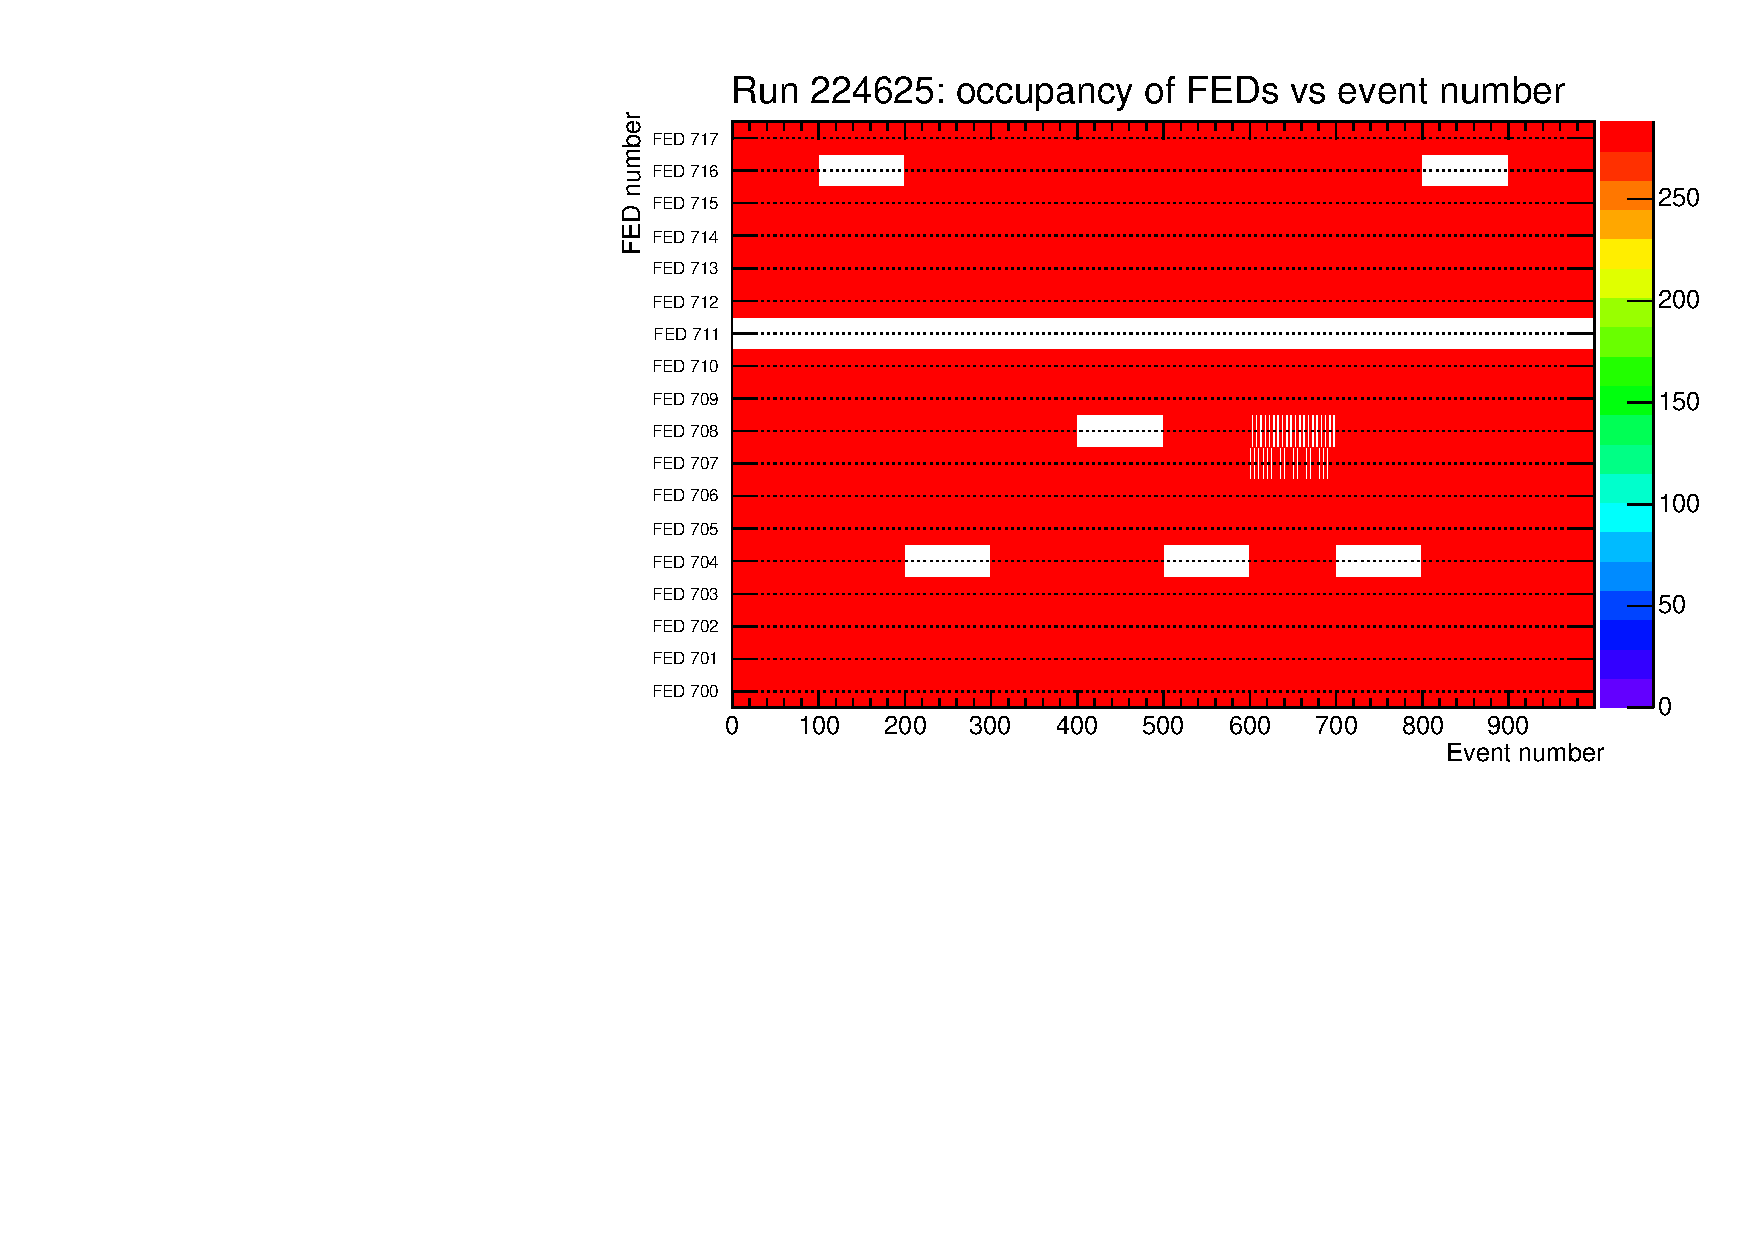
\includegraphics[width=.9\linewidth]{fig/fed_occ_vs_event_Run224625.pdf}
\end{column}
\begin{column}{0.55\textwidth}
%% Column 2
\label{sec-1-2-1-1-2}

\centering
\href{http://cmshcalweb01.cern.ch/DetDiag/Local_HTML/DQM_Hcal_R000224625_0/}{\alert{Run 224626}}
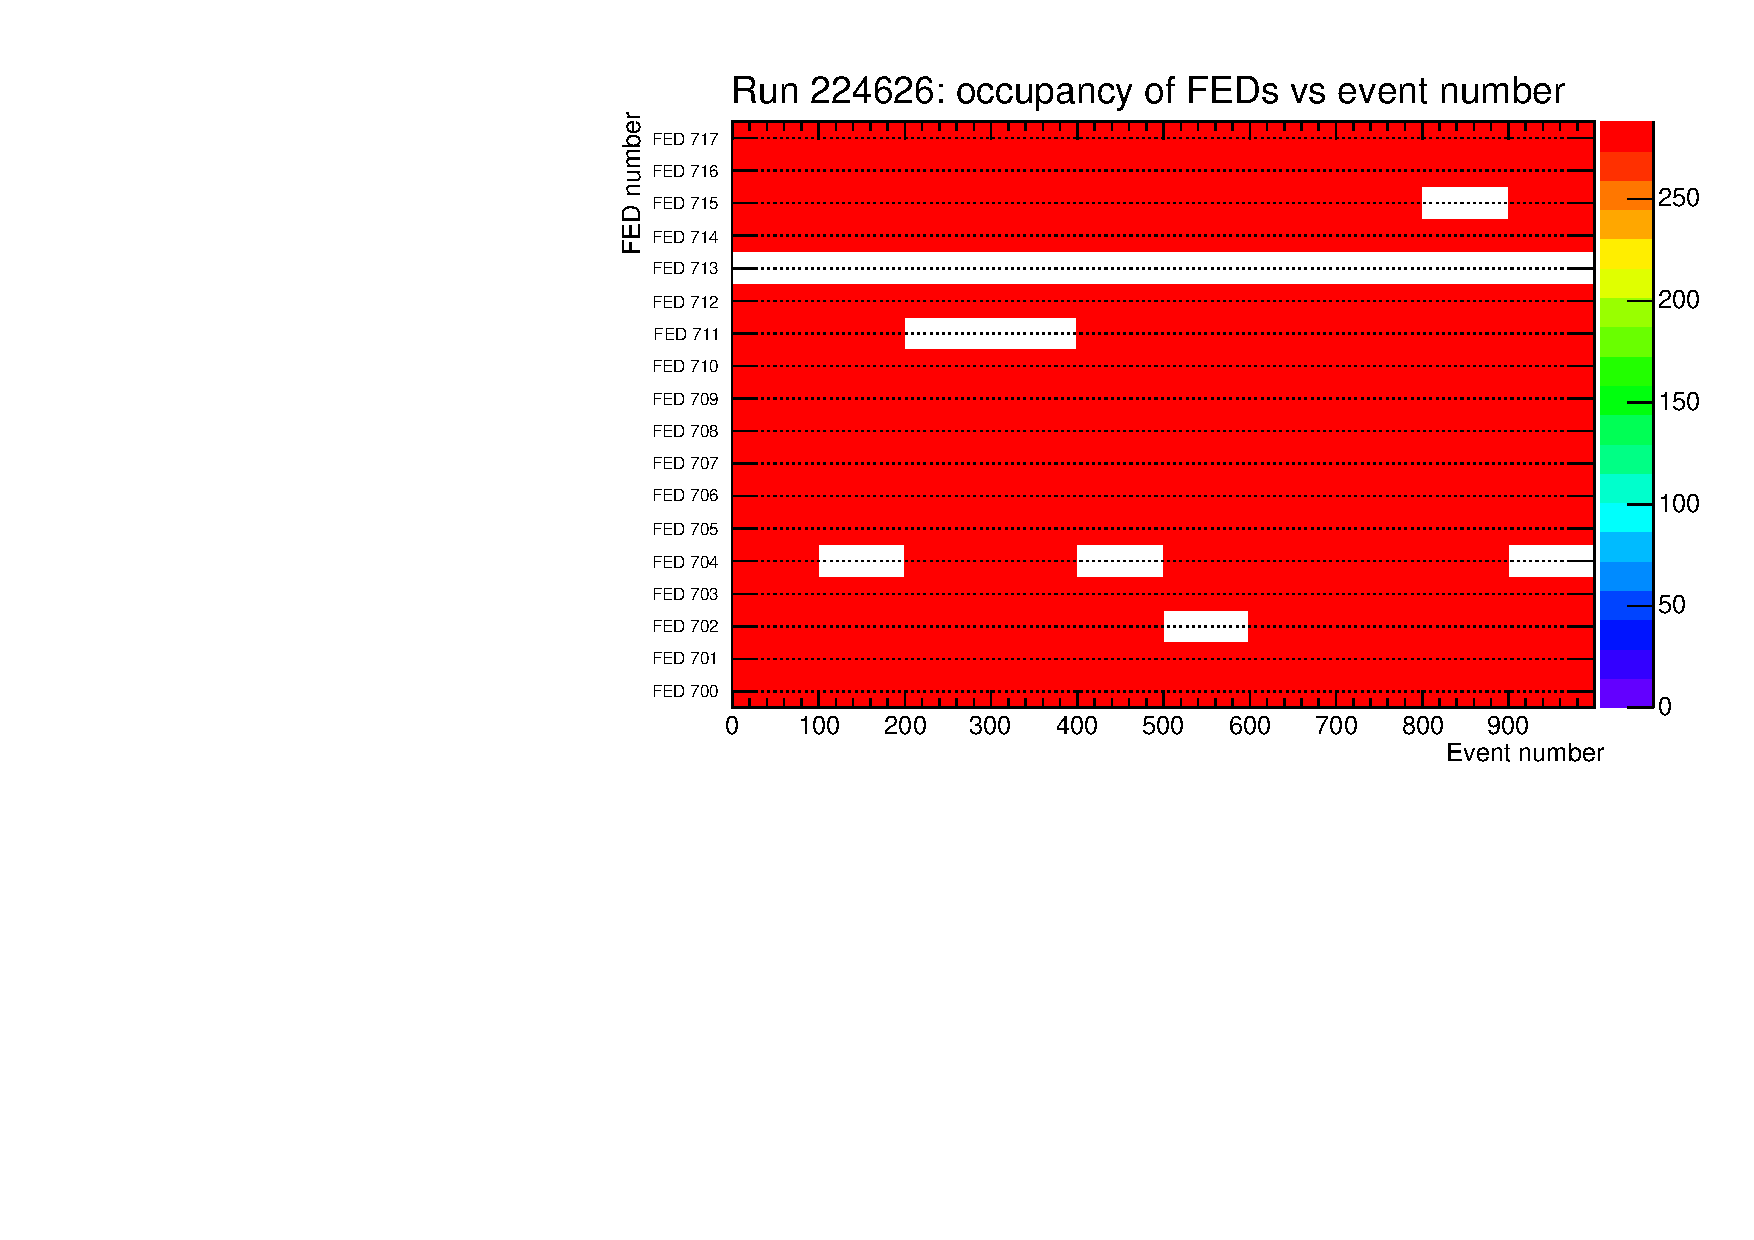
\includegraphics[width=.9\linewidth]{fig/fed_occ_vs_event_Run224626.pdf}
\end{column}
\end{columns}
\begin{itemize}

\item $x$-axis: Event number (1000 events in these runs)
\label{sec-1-2-1-2}%

\item $y$-axis: FED numbers
\label{sec-1-2-1-3}%

\item $z$-axis: Number of digis produced given FED \& event
\label{sec-1-2-1-4}%
\end{itemize} % ends low level
\end{frame}
\begin{frame}
\frametitle{Missing channels in HBHE laser runs}
\label{sec-1-2-2}
\begin{itemize}

\item Symptoms when FEDs are ``missing''
\label{sec-1-2-2-1}%
\begin{itemize}

\item No digis produced
\label{sec-1-2-2-1-1}%

\item FED data size = 0 bytes
\label{sec-1-2-2-1-2}%

\item Can't access FED headers
\label{sec-1-2-2-1-3}%
\end{itemize} % ends low level

\item Three kinds of failure:
\label{sec-1-2-2-2}%
\begin{enumerate}
\item Some FEDs drop out of laser runs entirely
\item Some FEDs drop out for 100 events at a time
\item Some FEDs ``flicker'' in and out of the run for 100 events
\end{enumerate}

\item Failure mode is unclear (to me, anyway):
\label{sec-1-2-2-3}%
\begin{itemize}

\item Are FEDs sporadically not being read out? (impossible?)
\label{sec-1-2-2-3-1}%

\item Are digis in these FEDs so bad that the unpacker won't unpack them?
\label{sec-1-2-2-3-2}%
\begin{itemize}

\item \texttt{hcalDigis.FilterDataQuality} set to \texttt{False}
\label{sec-1-2-2-3-2-1}%
\end{itemize} % ends low level
\end{itemize} % ends low level
\end{itemize} % ends low level
\end{frame}
\begin{frame}
\frametitle{Missing channels in HBHE laser runs}
\label{sec-1-2-3}
\begin{itemize}

\item DAQ logs have the following errors:
\label{sec-1-2-3-1}%
\begin{itemize}

\item \texttt{ERROR Caught exception: hcal:\textbf{:exception:}:Exception 'Expected 100 events, saw 32 from QDC 0' raised at readout(hcalQDCTDCReadout.cc:209)}
\label{sec-1-2-3-1-1}%

\item \texttt{WARN Chunk received for unknown source 711}
\label{sec-1-2-3-1-2}%
\end{itemize} % ends low level
\end{itemize} % ends low level
\end{frame}
\begin{frame}
\frametitle{Missing channels in HBHE laser runs}
\label{sec-1-2-4}
\begin{itemize}

\item Investigation continues:
\label{sec-1-2-4-1}%
\begin{itemize}

\item DAQ expert (Chris West) investigating
\label{sec-1-2-4-1-1}%

\item Currently only see these problems in HBHE laser runs
\label{sec-1-2-4-1-2}%
\begin{itemize}

\item Looking in other run types too
\label{sec-1-2-4-1-2-1}%
\end{itemize} % ends low level
\end{itemize} % ends low level
\end{itemize} % ends low level
\end{frame}

\end{document}
